% -*- program: xelatex -*-
%\documentclass[12pt, compress]{beamer} 
\documentclass[12pt, compress]{beamer}       
%\documentclass[notes=only]{beamer}

\usepackage{fontspec}
	
\setsansfont{PT Sans}
\setmonofont{Liberation Mono}

\usepackage{beamerthemesplit}
\usefonttheme[onlymath]{serif}
%\DeclareFontEncoding{T1}
\fontencoding{T1}

%\usepackage[T2A]{fontenc} 
%\usepackage[utf8x]{inputenc}
\usepackage[russian]{babel}
\usepackage{listings}

\usepackage{amsmath,amssymb,amsthm} 
\hypersetup{unicode=true}
\usepackage{graphics,graphicx}
\usepackage{verbatim} 
\usepackage{fancyvrb}
\usepackage{booktabs}
\usepackage{media9}
\usepackage[super]{natbib}
\usepackage{color}
\definecolor{mygreen}{RGB}{28,172,0} % color values Red, Green, Blue
\definecolor{mylilas}{RGB}{170,55,241}
\definecolor{codecolor}{RGB}{0,120,0}
\definecolor{light-gray}{gray}{0.95}
\definecolor{light-green}{rgb}{0.93, 1, 0.8}
\definecolor{light-yellow}{rgb}{1,1,0.85}
\definecolor{dark-blue}{rgb}{0,0,0.6}
\definecolor{dark-red}{rgb}{0.7,0,0.0}
\definecolor{dark-green}{RGB}{10,150,0}
\definecolor{ssau-color}{RGB}{0,163,224}

\usepackage{pifont}% http://ctan.org/pkg/pifont
\newcommand{\cmark}{\textcolor{green}{\ding{51}}}
\newcommand{\xmark}{\textcolor{red}{\ding{55}}}

\setbeamercolor{frametitle}{fg=ssau-color,bg=gray!10}
\setbeamerfont{title}{series=\bfseries,parent=structure}
\setbeamerfont{frametitle}{series=\bfseries,parent=structure}

\setbeamertemplate{blocks}[rounded][shadow=false]
\setbeamertemplate{navigation symbols}{}

\newcommand{\code}[1]{\textcolor{dark-green}{\texttt{#1}}}
\newcommand{\cleartitlepage}[1]{\begin{frame}[plain]\begin{center}\textsc{#1}\end{center}\end{frame}}
\renewcommand{\emph}[1]{\textcolor{dark-blue}{#1}}
\newcommand{\emphb}[1]{\textcolor{dark-blue}{\textbf{#1}}}
\newcommand{\lstcomment}[1]{\textcolor{dark-green}{\# \texttt{#1}}}

\usepackage{dirtree}

\usetheme{CambridgeUS}
\usecolortheme{lily}

\lstset{basicstyle=\ttfamily,
    language=gnuplot,    
    keepspaces=true,
    extendedchars=\true,
    basicstyle={\small},
    breaklines=true,
    morekeywords={matlab2tikz},
    keywordstyle=\color{blue},
    morekeywords=[2]{1}, keywordstyle=[2]{\color{blue}},
    identifierstyle={ \bf \color{black} },
    stringstyle=\color{mylilas},
    commentstyle=\color{mygreen},%
    showstringspaces=false,
    numbers=left,%
    numberstyle={\scriptsize \color{gray}},
    numbersep=7pt, 
    emph=[1]{case,switch,otherwise,nonlocal,as,yield, with},emphstyle=[1]\color{blue}, 
    frame=single,    
    rulecolor=\color{red},    
    backgroundcolor=\color{light-gray},
    xleftmargin=0.3cm,
    frame=l,framesep=4pt,framerule=0.5pt,
    escapechar=|
    %lineskip=-1.0pt,
    %emph=[2]{word1,word2}, emphstyle=[2]{style},    
}

\usepackage{tikz}
\usetikzlibrary{positioning} 
\tikzset{cbutton/.style={rectangle,minimum width=10mm,thick,draw=red!50!black!50,
top color=white,bottom color=red!50!black!30}}
\tikzset{mbutton/.style={rectangle,minimum width=10mm,thick,draw=black!20,
top color=white,bottom color=black!30}}

\usetikzlibrary{arrows,shapes}
\tikzstyle{every picture}+=[remember picture]

\setbeamercolor*{palette primary}{use=structure,fg=white,bg=ssau-color}
\setbeamercolor*{palette secondary}{fg=ssau-color,bg=gray!15!white}
\setbeamercolor*{palette tertiary}{use=structure,fg=white,bg=ssau-color}
\setbeamercolor*{palette quaternary}{fg=ssau-color,bg=gray!5!white}
\setbeamercolor{frametitle}{fg=white,bg=ssau-color}

\makeatother
\setbeamertemplate{footline}
{
  \leavevmode%
  \hbox{%  
  \begin{beamercolorbox}[wd=.3\paperwidth,ht=2.25ex,dp=1ex,center]{author in head/foot}%
    \usebeamerfont{author in head/foot}\insertshortauthor
  \end{beamercolorbox}%  
  \begin{beamercolorbox}[wd=.6\paperwidth,ht=2.25ex,dp=1ex,center]{title in head/foot}%
    \usebeamerfont{title in head/foot}\insertshorttitle
  \end{beamercolorbox}%
  \begin{beamercolorbox}[wd=.1\paperwidth,ht=2.25ex,dp=1ex,center]{date in head/foot}%
   %\insertframenumber{} / \inserttotalframenumber\hspace*{1ex}
    \insertframenumber{} 
  \end{beamercolorbox}}%
  \vskip0pt%
}

\setbeamertemplate{headline}{}
%\setbeamertemplate{footline}{}
 
\AtBeginSection[]{
  \begin{frame}[plain]
  %\vfill  
  \begin{tikzpicture}
  \useasboundingbox (0,0) rectangle(\the\paperwidth,\the\paperheight);  
  \fill[color=ssau-color]   (-1cm, 3.9cm) rectangle(\the\paperwidth, 5.9cm);
  %\usebeamerfont{title}\insertsectionhead\par%
  %\node[text width=\the\paperwidth,align=center] at (current page.center) {\color{ExecusharesWhite}\Large\textbf{\insertsectionhead}};  
  \node[text width=\the\paperwidth,align=center] at (6cm,4.9cm) {\color{white}\Large\textbf{\insertsectionhead}};  
  \end{tikzpicture}
  \end{frame}
}



% ============================================================================

\title[Основы GNUPLOT]{Основы GNUPLOT}
\subtitle{Компьютерная графика}
\author[Самарский университет]{Юдинцев В. В.}
\institute{Кафедра теоретической механики}
\date{\today}

\usepackage{tikz}
\usetikzlibrary{positioning} 
\tikzset{cbutton/.style={rectangle,minimum width=10mm,thick,draw=red!50!black!50,
top color=white,bottom color=red!50!black!30}}
\tikzset{mbutton/.style={rectangle,minimum width=10mm,thick,draw=black!20,
top color=white,bottom color=black!30}}


\tikzstyle{block} = [rectangle, draw, fill=yellow!20, text width=5em, text centered, rounded corners, minimum height=5em]
\tikzstyle{subblock} = [rectangle, draw, fill=white, text width=2em, text centered, minimum height=1em]
\tikzstyle{module} = [rectangle, draw, fill=none, text width=5em, text centered, rounded corners, minimum height=5em]
\tikzstyle{line} = [draw, ->]

\usepackage{menukeys}

\begin{document}

{
\setbeamercolor{background canvas}{bg=white} 
\usebackgroundtemplate{
\includegraphics[width=\paperwidth,height=\paperheight]{back.png}}
\begin{frame}[plain]
%\begin{figure}[h]
%  \centering
  %\includegraphics[width=0.3\textwidth]{}
%\end{figure}
\maketitle
\end{frame}
}

%
% \frame{\frametitle{Содержание}\tableofcontents}
%

\begin{frame}[c]
\frametitle{GNUPLOT}
\begin{itemize}
\item \emph{свободная} программа для создания двухмерных и трёхмерных графиков в командном интерактивном режиме или в режиме выполнения команд из файла
\item результат работы программы -- изображение на экране или графический файл (.eps, .png, .pdf, ...)
\item работает на всех основых платформах: Linux, Microsoft Windows, macOS
\item первая версия программы вышла в 1986 году
\item используется в качестве системы вывода изображений в различных свободных математических пакетах: GNU Octave, Maxima
\end{itemize}
\end{frame}

\begin{frame}[c]
\frametitle{Установка}
\url{http://www.gnuplot.info/}
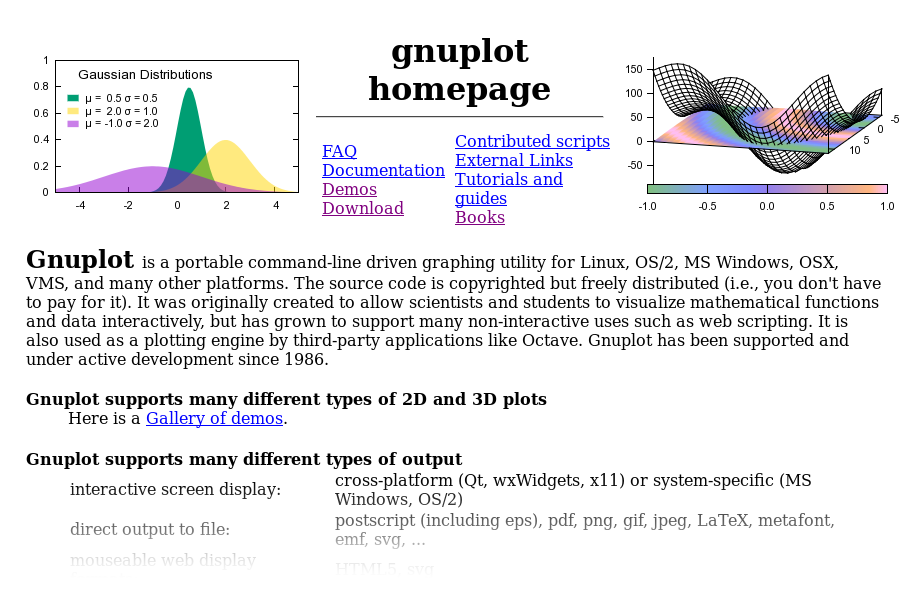
\includegraphics[width=1.0\textwidth]{gnuplot.png}
\end{frame}

\begin{frame}[c]
\frametitle{Установка}
{\tiny
\url{https://sourceforge.net/projects/gnuplot/files/gnuplot/5.2.2/}
}
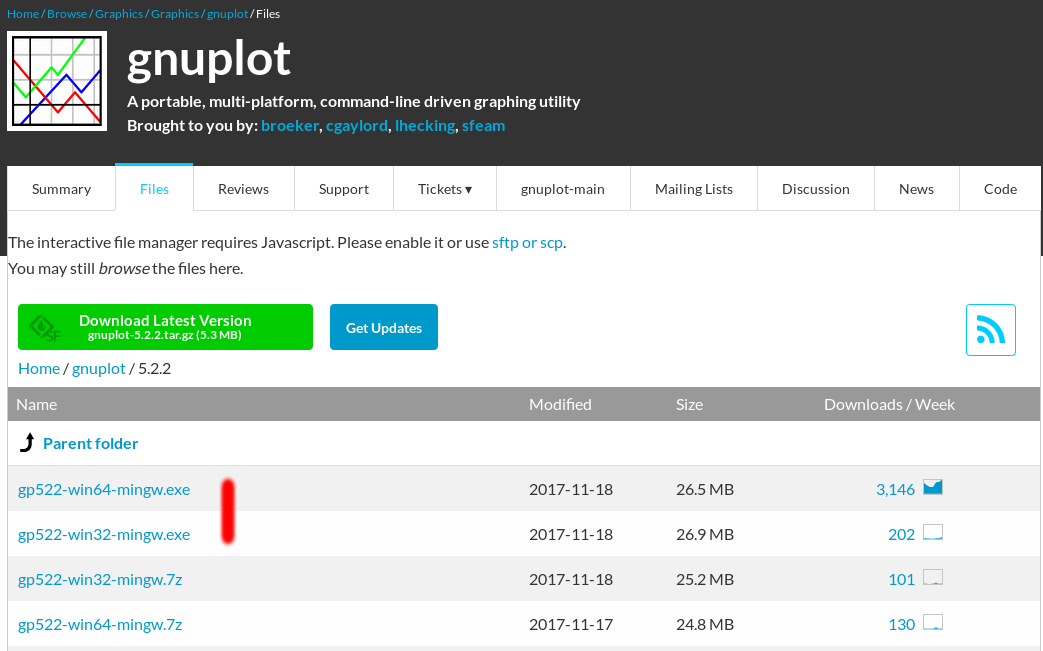
\includegraphics[width=1.0\textwidth]{install.png}
\end{frame}

\begin{frame}[t]
\frametitle{Информация}
\begin{columns}
\column{0.5\linewidth}

\includegraphics[width=1.0\textwidth]{book.png}\\
\column{0.5\linewidth}
Philipp K. Janert 

\emph{Gnuplot in Action}

Second Edition

2016. 400 с.
\end{columns}  
\end{frame}


\begin{frame}[t]
\frametitle{Информация}
\begin{itemize}
  \item[en] Страница проекта \\
  {\scriptsize \url{http://www.gnuplot.info/} }
  \item[en] Примеры \\
  {\scriptsize \url{http://gnuplot.sourceforge.net/demo_5.2/} }
  \item[en] Руководство пользователя \\
  {\scriptsize  \url{http://www.gnuplot.info/docs_5.2/Gnuplot_5.2.pdf} }
  \item[ru] Нечаев А. Н. Краткое введение в GNUPLOT \\
  {\scriptsize  \url{http://www.phys.vsu.ru/~meremianin/pdfs/gnuplot-gdoc.pdf} }
  \item[ru] Построение научных и инженерных графиков с помощью GNUPLOT \\
  {\scriptsize  \url{https://www.ibm.com/developerworks/ru/library/l-GnuPlot_01/} }  
\end{itemize}
\end{frame}


\begin{frame}[c]
\frametitle{Спообы работы: диалоговый режим}
\begin{figure}[htbp]
	\centering
	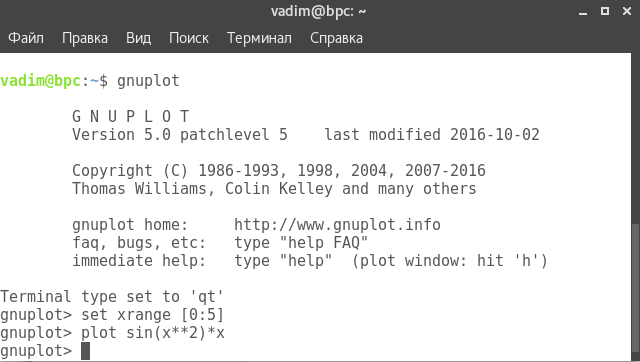
\includegraphics[width=0.95\textwidth]{simple_command.png}
\end{figure}
\end{frame}
 
\begin{frame}[c]
\frametitle{Диалоговый режим}
\begin{figure}[htbp]
	\centering
	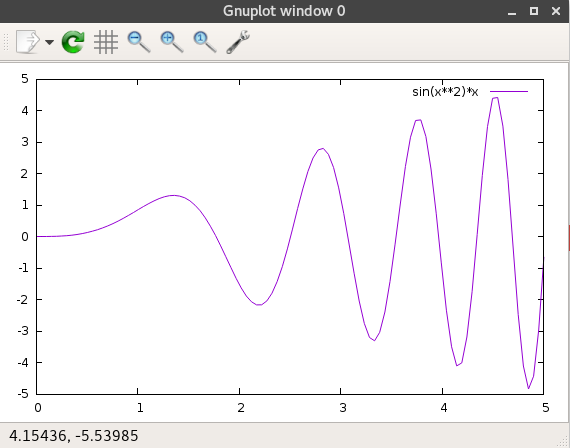
\includegraphics[width=0.8\textwidth]{simple_command_result.png}
\end{figure}
\end{frame}


\begin{frame}[c,fragile]
\frametitle{Файл-сценарий plot.gp}
В текстовом редакторе (Блокнот, atom, sublimetext, ...) создаётся файл с инструкциями (командами) для gnuplot
\begin{lstlisting}
|\lstcomment{Способ вывода}|
set term pngcairo size 1200,800 font 'Times,26'
|\lstcomment{Файл с результатом}|
set output 'plot1.png'
|\lstcomment{Подписи осей}|
set xlabel "t, c"
set ylabel "y, м"
set title "Движение точки"
|\lstcomment{Диапазон для горизонтальной оси}|
set xrange [0:2]
plot sin(x) title 'Перемещение'
\end{lstlisting}
Для выполнения скрипта в терминале вызывается программа gnuplot с параметром -- именем файла: \code{gnuplot plot.gp}
\end{frame}

\begin{frame}[c,fragile]
\frametitle{Результат работы программы -- \emph{plot1.png}}
\begin{figure}
  \centering
  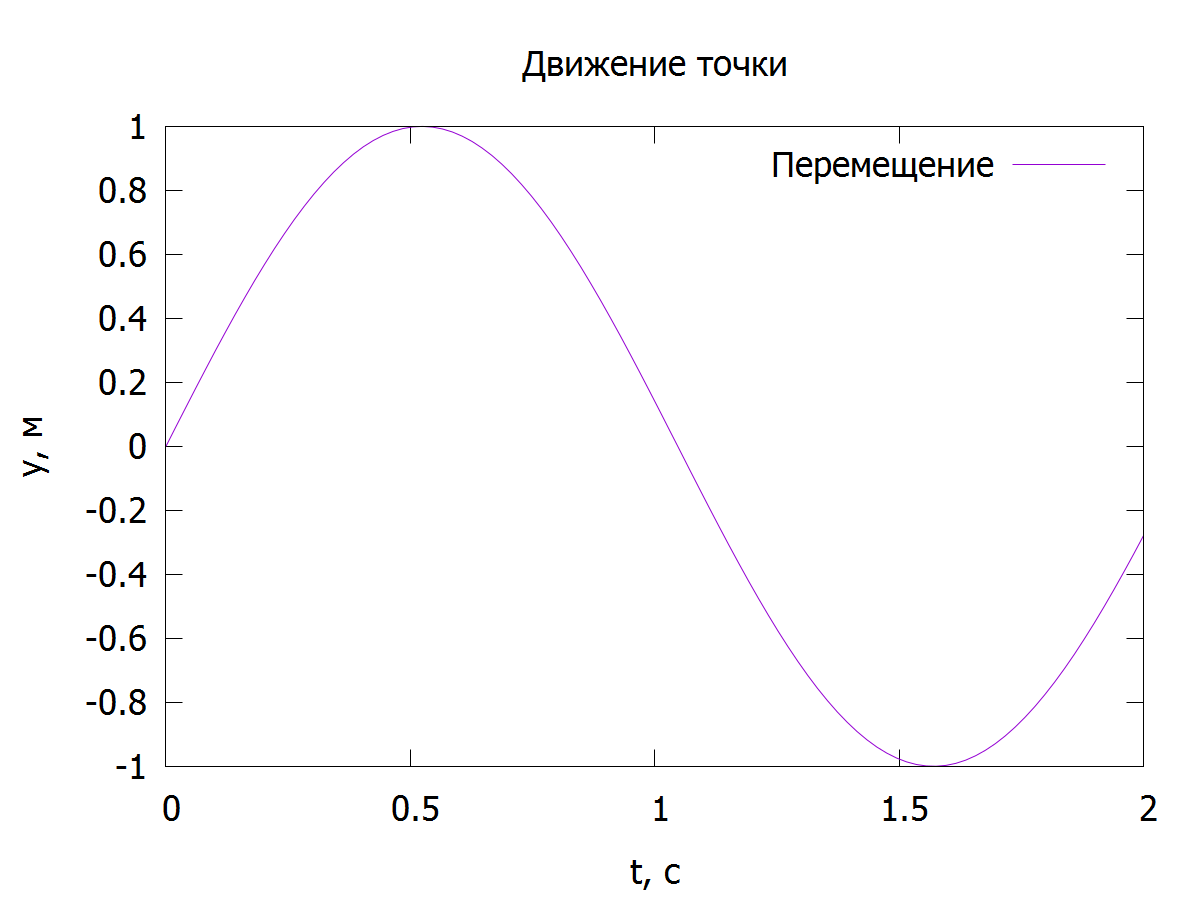
\includegraphics[width=0.85\textwidth]{./gp/plot1.png}
\end{figure}
\end{frame}

\section{Способы и параметры вывода}

\begin{frame}[c]
\frametitle{set terminal}
Команда \emph{set terminal} определяет способ вывода результата работы программы \emph{gnuplot}:
\begin{itemize}
  \item на экран
  \item в растровый файл \emph{png}
  \item в векторный файл \emph{pdf}, \emph{eps}, \emph{svg}, \emph{epslatex}
\end{itemize}
\end{frame}


\begin{frame}[c,fragile]
\frametitle{Формат png: \emph{set terminal pngcairo}}
\emph{pngcairo} -- терминал для вывода в растровый графический формат \emph{.png}.

\vspace{10pt}
\begin{itemize}
\item Размер изображения 640x480 точек шрифт 12 точек
\begin{lstlisting}
set terminal pngcairo font 'Arial,12'
\end{lstlisting}
\item Размер изображения 1200x900 точек шрифт 26
\begin{lstlisting}
set terminal pngcairo size 1200,900 \ 
             font 'Times,26'
\end{lstlisting}
\item Базовая толщина линий
\begin{lstlisting}
set terminal pngcairo size 1200,900 \ 
             font 'Times,26' linewidth 2
\end{lstlisting}
\end{itemize}
\end{frame}

\begin{frame}[c,fragile]
\frametitle{Формат svg: \emph{set terminal svg}}
\emph{pngcairo} -- терминал для вывода в векторный графический формат \emph{.svg}.

\vspace{10pt}
\begin{itemize}
\item Размер изображения 640x480 точек шрифт 12 точек
\begin{lstlisting}
set terminal svg font 'Arial,12'
\end{lstlisting}
\item Размер изображения 1200x900 точек шрифт 26
\begin{lstlisting}
set terminal svg size 1200,900 \ 
             font 'Times,26'
\end{lstlisting}
\item Базовая толщина линий
\begin{lstlisting}
set terminal svg size 1200,900 \ 
             font 'Times,26' linewidth 2
\end{lstlisting}
\end{itemize}
\end{frame}


\begin{frame}[c,fragile]
\frametitle{Формат pdf}
\emph{pdfcairo} -- терминал для вывода в векторный графический формат \emph{.pdf}.

\vspace{10pt}
\begin{itemize}
\item Размер изображения 5x3 дюйма шрифт 12*(1/72) мм
\begin{lstlisting}
set terminal pdfcairo font 'Arial,12'
\end{lstlisting}
\item Размер изображения 6x5 дюйма шрифт 26*(1/72) мм
\begin{lstlisting}
set terminal pdfcairo size 6,5 \ 
             font 'Times,26'
\end{lstlisting}
\item Базовая толщина линий 2
\begin{lstlisting}
set terminal pdfcairo size 6,5 \ 
             font 'Times,26' linewidth 2
\end{lstlisting}
\end{itemize}
\end{frame}


\section{Графики функций}


\begin{frame}[c,fragile]
\frametitle{Функции}
\begin{lstlisting}
set term pngcairo size 1200,800 font "Times,26" \
    linewidth 2
|\lstcomment{Диапазон x}|
set xrange [-5:5]
|\lstcomment{Диапазон y}|
set yrange [-1.5:1.5]
|\lstcomment{Подписи осей}|
set xlabel 'x'
set ylabel 'f'
|\lstcomment{Файл вывода}|
set output 'functions.png'

plot sin(x) with linespoints,\
     cos(x) with linespoints
\end{lstlisting}
\end{frame}


\begin{frame}[c,fragile]
\frametitle{Функции}
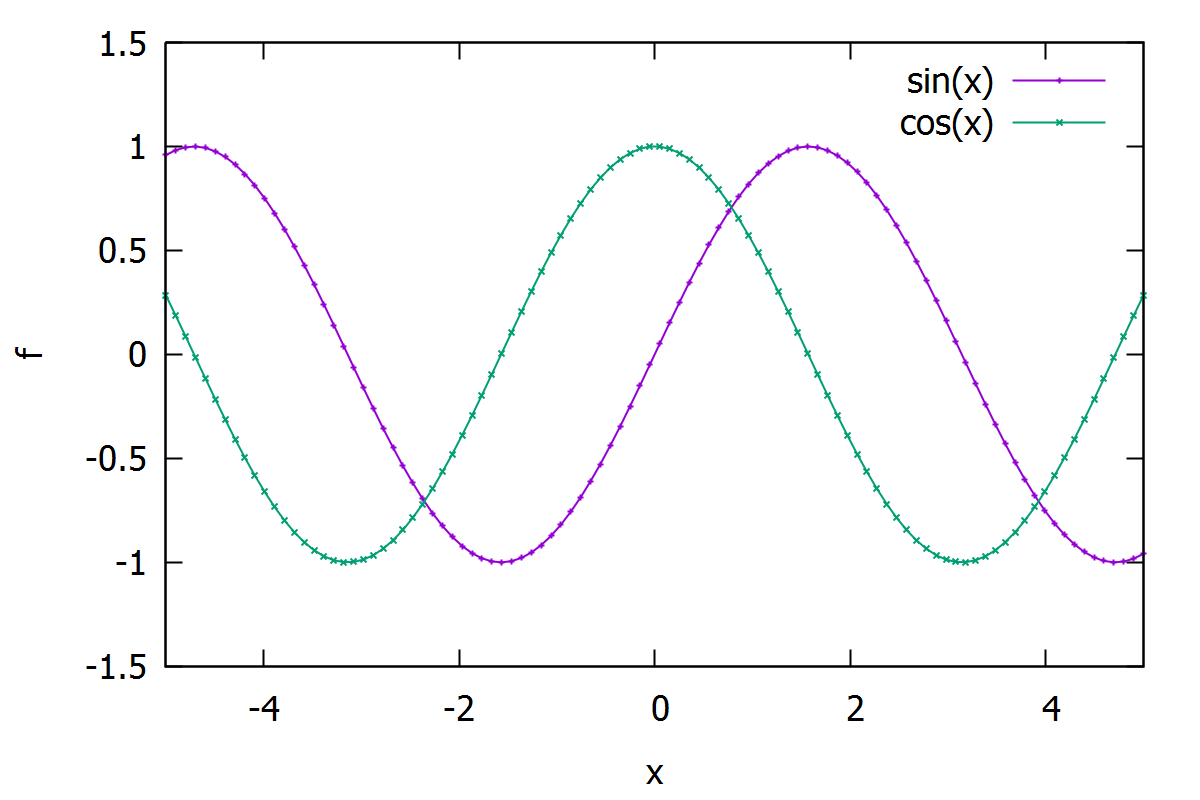
\includegraphics[width=0.95\textwidth]{./gp/functions1.png}
\end{frame}

\begin{frame}[c,fragile]
\frametitle{Линии без маркеров}
\begin{lstlisting}
set term pngcairo size 1200,800 font "Times,26" \
    linewidth 2
|\lstcomment{Диапазон x}|
set xrange [-5:5]
|\lstcomment{Диапазон y}|
set yrange [-1.5:1.5]
|\lstcomment{Подписи осей}|
set xlabel 'x'
set ylabel 'f'
|\lstcomment{Файл вывода}|
set output 'functions.png'

plot sin(x) with lines,\
     cos(x) with lines
\end{lstlisting}
\end{frame}

\begin{frame}[c,fragile]
\frametitle{Линии без маркеров}
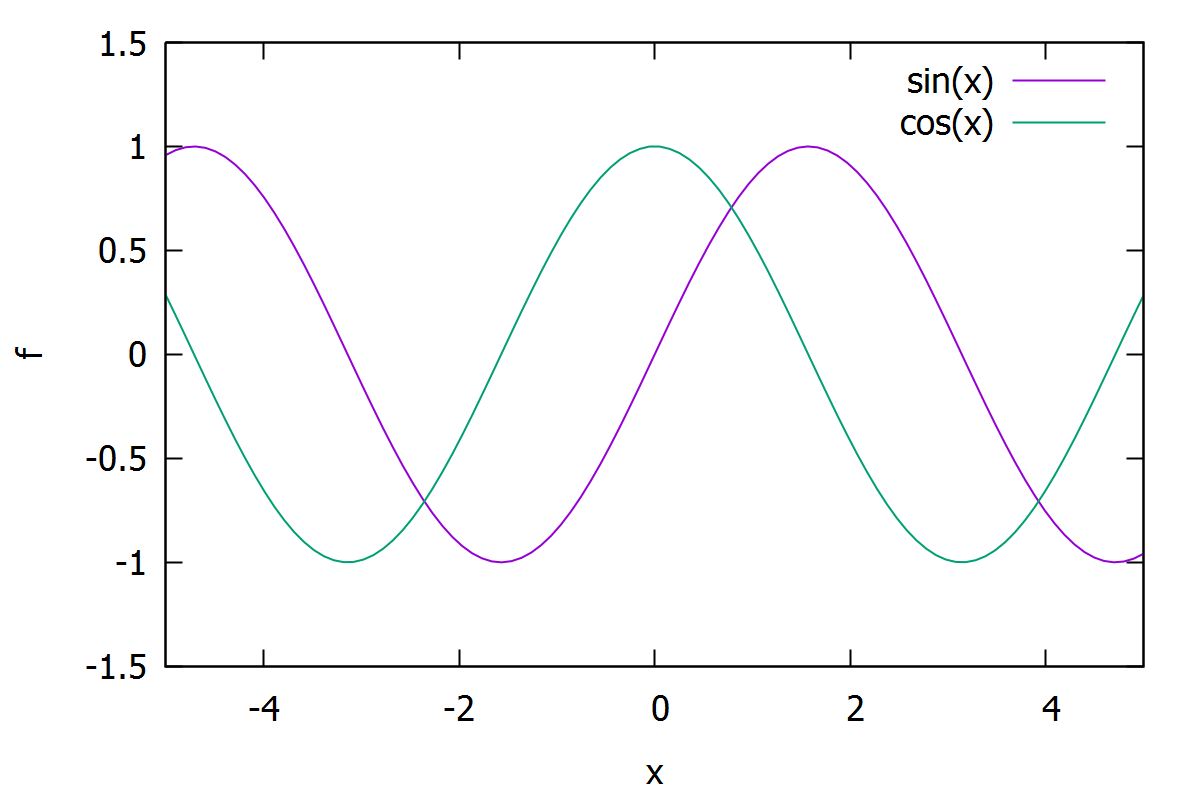
\includegraphics[width=0.95\textwidth]{./gp/functions2.png}
\end{frame}


\begin{frame}[c,fragile]
\frametitle{Линии, маркеры, линии с маркерами}
\begin{lstlisting}
set term pngcairo size 1200,800 font "Times,26" linewidth 2

set output 'line_style.png'

set xrange [-5:5]
set yrange [-1.5:1.5]
set xlabel 'x'
set ylabel 'f'

plot sin(x) with lines, \
     cos(x) with points, \
     0.5*x  with linespoints
\end{lstlisting}
\end{frame}

\begin{frame}[t]
\frametitle{Стили графика}
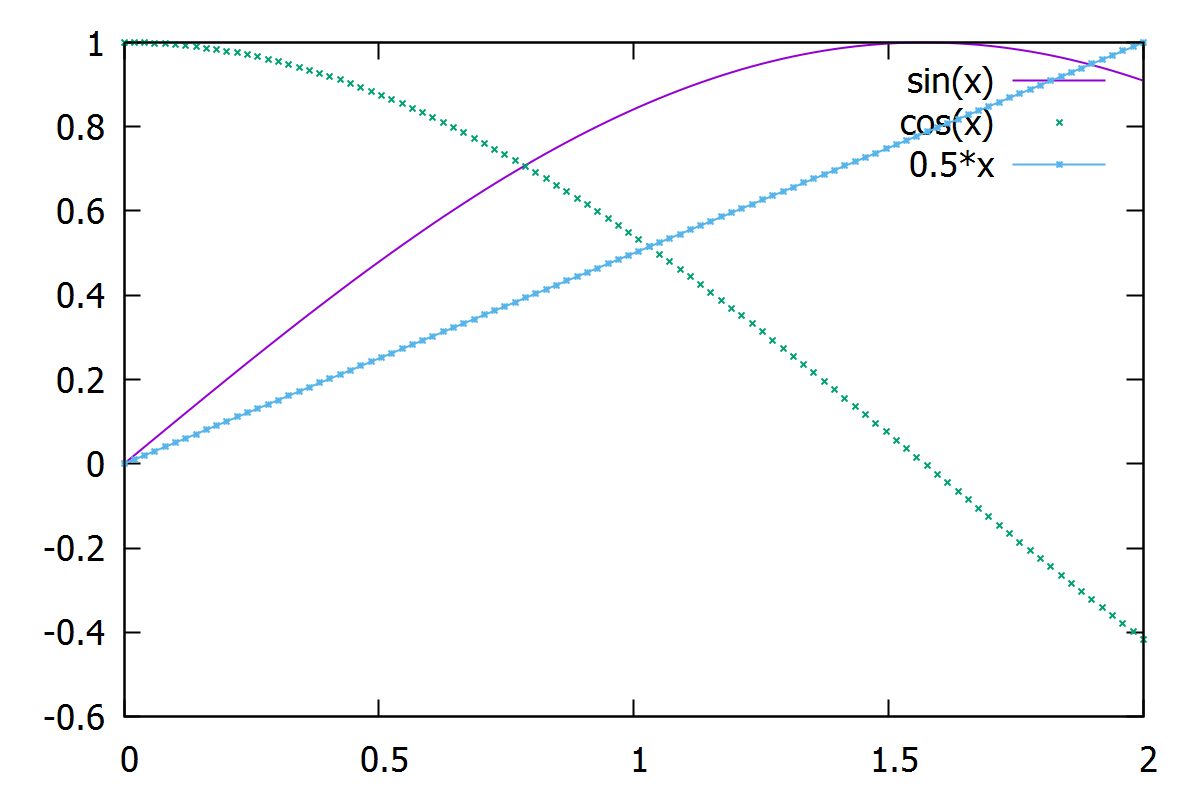
\includegraphics[width=0.98\textwidth]{./gp/line_style.png}
\end{frame}

\begin{frame}[c,fragile]
\frametitle{Подпись данных (легенда)}
\begin{lstlisting}
set term pngcairo size 1200,800 font "Times,26" \
    linewidth 2

set key top, left

set xrange [-5:5]
set yrange [-1.5:1.5]
set xlabel 'x'
set ylabel 'f'

set output 'functions.png'

plot sin(x) title 'Синус' with lines,\
     cos(x) title 'Косинус' with lines
\end{lstlisting}
\end{frame}

\begin{frame}[c,fragile]
\frametitle{Подпись данных (легенда)}
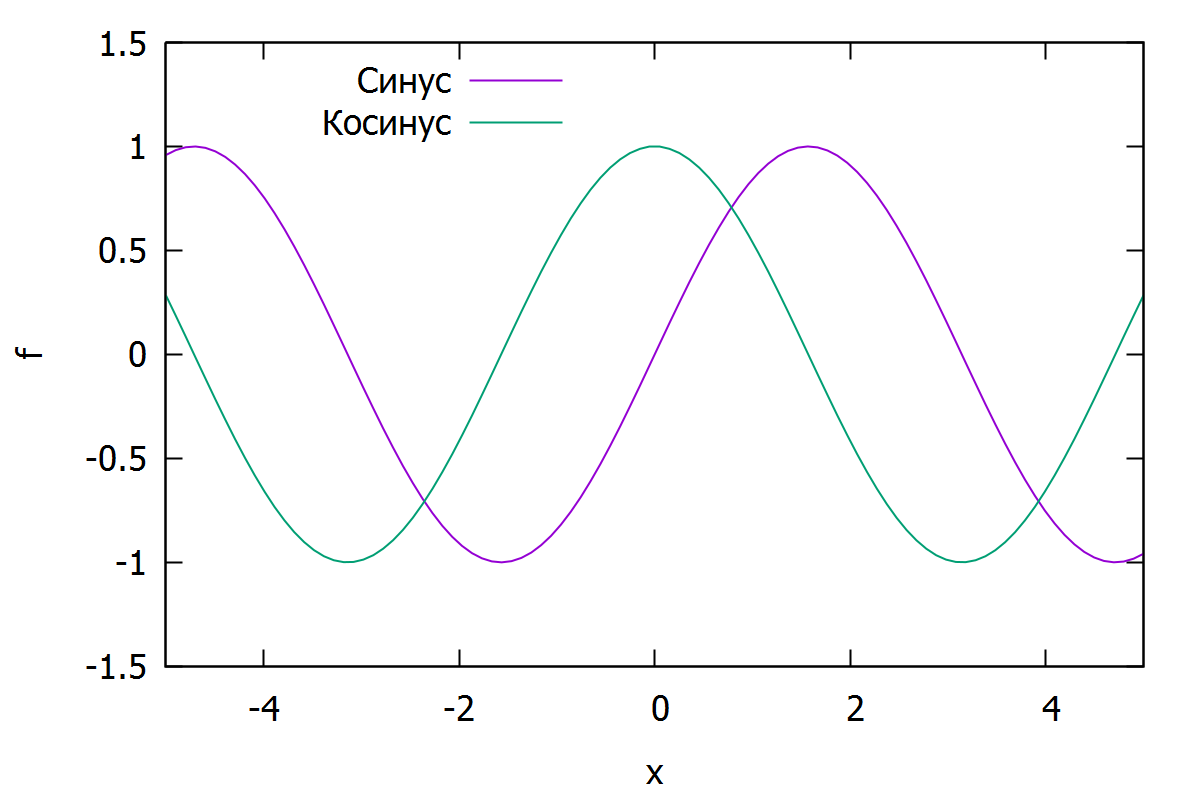
\includegraphics[width=0.95\textwidth]{./gp/functions3.png}
\end{frame}

\begin{frame}[c,fragile]
\frametitle{Тип линии}
\begin{lstlisting}
set term pngcairo size 1200,800 font "Times,26" \
    linewidth 3

set output 'line_style_line.png' 

set xrange [-5:5]
set yrange [-1.5:1.5]
set xlabel 'x'
set ylabel 'f'

plot sin(x) with lines, \
     cos(x) with lines dt '-', \
     0.5*x  with lines dt '_'
\end{lstlisting}
\end{frame}

\begin{frame}[c,fragile]
\frametitle{Тип линии}
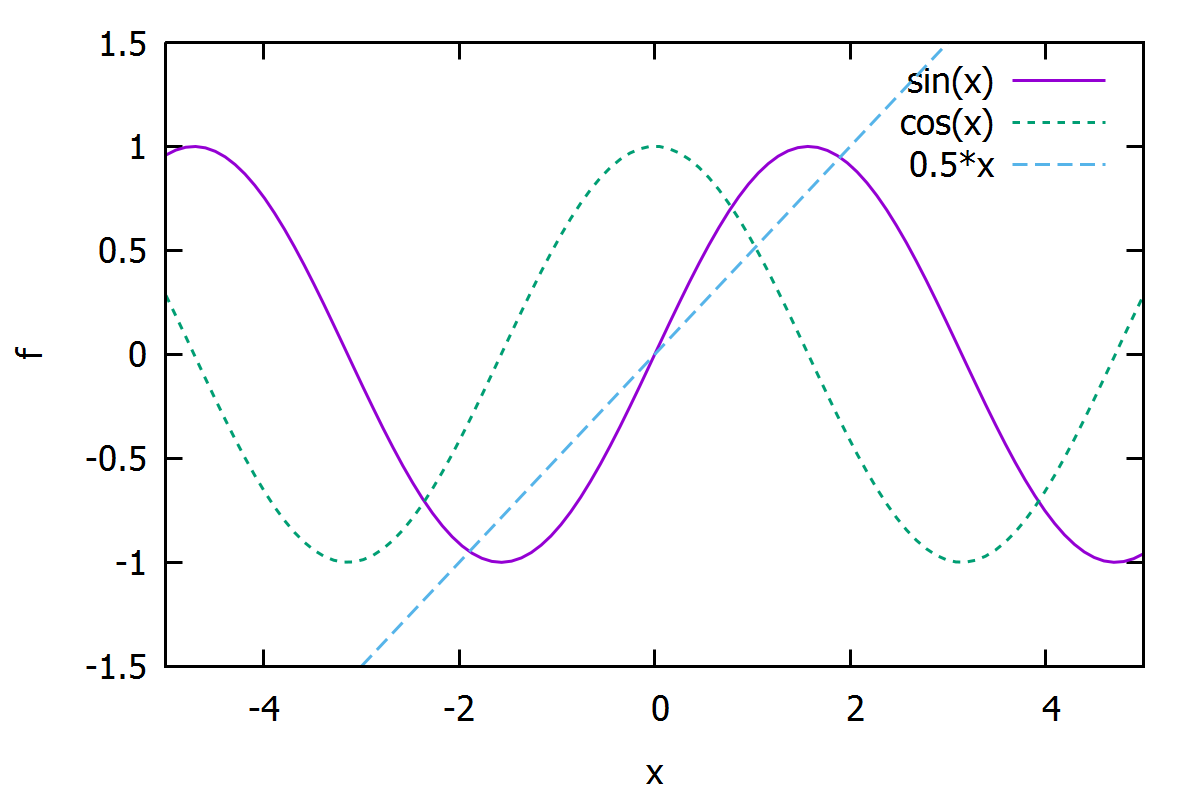
\includegraphics[width=0.95\textwidth]{./gp/line_style_line.png}
\end{frame}

\begin{frame}[c,fragile]
\frametitle{Создание стиля линии}
Стиль линии -- это сочетание её свойств:
\begin{itemize}
  \item толщина;
  \item тип (сплошная, пунктирная, ...);
  \item цвет;
  \item типа маркера.
\end{itemize}
Красная линия толщиной 2, без маркера
\begin{lstlisting}
set style line 1 lw 2 lc rgb 'red'   pt 1
\end{lstlisting}
Зелёная и синяя с маркерами типа 2 и 3
\begin{lstlisting}
set style line 2 lw 2 lc rgb 'green' pt 2
set style line 3 lw 2 lc rgb 'blue'  pt 3
\end{lstlisting}
\end{frame}

\begin{frame}[t,fragile]
\frametitle{Тип маркера}
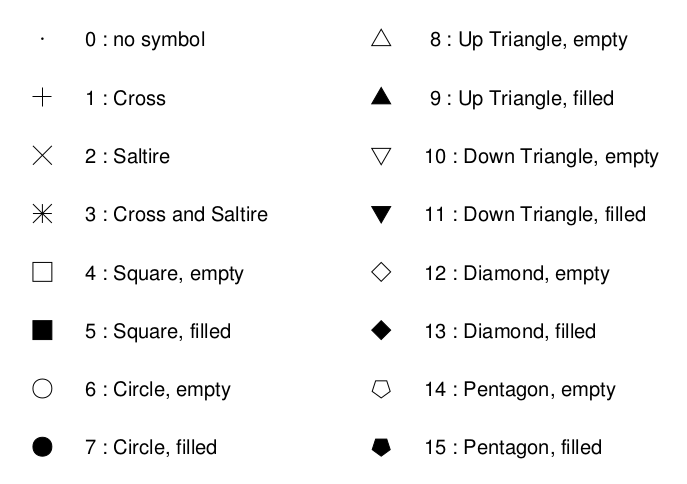
\includegraphics[width=0.9\textwidth]{marker_types.png}
\end{frame}

\begin{frame}[t,fragile]
\frametitle{Пример}
Свойство линии \code{pointinterval} регулирует 'частоту' маркеров
\begin{lstlisting}[basicstyle={\scriptsize}]
set term pngcairo size 1200,800 font "Times,26" linewidth 2

set style line 1 lw 2 lc rgb 'red'   pt 0 
set style line 2 lw 2 lc rgb 'green' pt 4  ps 2
set style line 3 lw 2 lc rgb 'blue'  pt 10 ps 2 pointinterval 4    

set output 'custom_lines_style.png'

set xrange [-5:5]
set yrange [-1.5:1.5]
set xlabel 'x'
set ylabel 'f'

plot sin(x) t '{/Symbol f}' with lines       ls 1 ,\
     cos(x) t 'x'           with linespoints ls 2 ,\
     0.5*x  t '{/Symbol w}' with linespoints ls 3
\end{lstlisting}  
\end{frame}

\begin{frame}[t,fragile]
\frametitle{Пример}
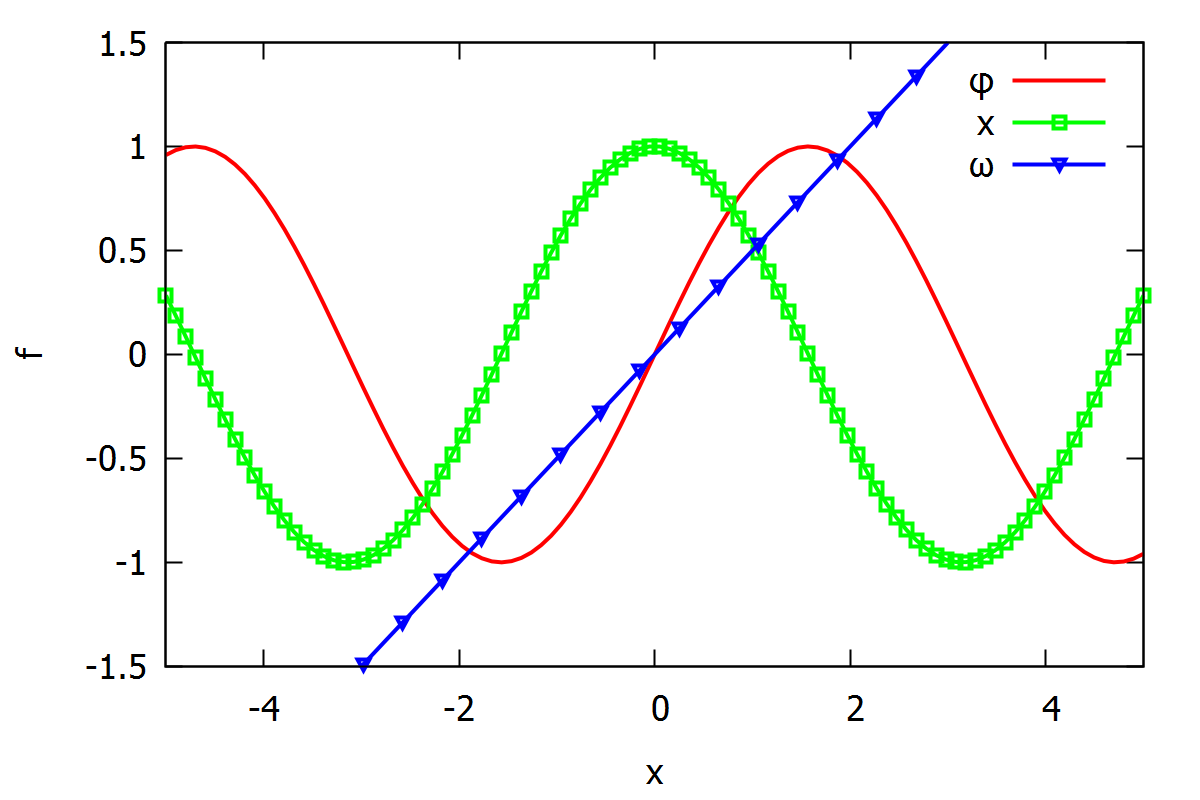
\includegraphics[width=0.95\textwidth]{./gp/custom_lines_style.png}
\end{frame}


\begin{frame}[t,fragile]
\frametitle{Монохромные графики}
Для подготовки графиков к монохромной печати можно определить собственные стили линий 
\begin{lstlisting}[basicstyle={\scriptsize}]
set term pngcairo size 1200,800 font "Times,26" linewidth 2

set style line 1 lw 2 lc -1 pt 1 
set style line 2 lw 2 lc -1 pt 2 dt (10,4)
set style line 3 lw 2 lc -1 pt 3 dt (10,4,4,4)

set output 'custom_lines_style_dashed.png'

set xrange [-5:5]
set yrange [-1.5:1.5]
set xlabel 'x'
set ylabel 'f'

plot sin(x) t '{/Symbol f}' with lines ls 1 ,\
     cos(x) t 'x'           with lines ls 2 ,\
     0.5*x  t '{/Symbol w}' with lines ls 3

\end{lstlisting}
\end{frame}

\begin{frame}[t,fragile]
\frametitle{Монохромные графики}
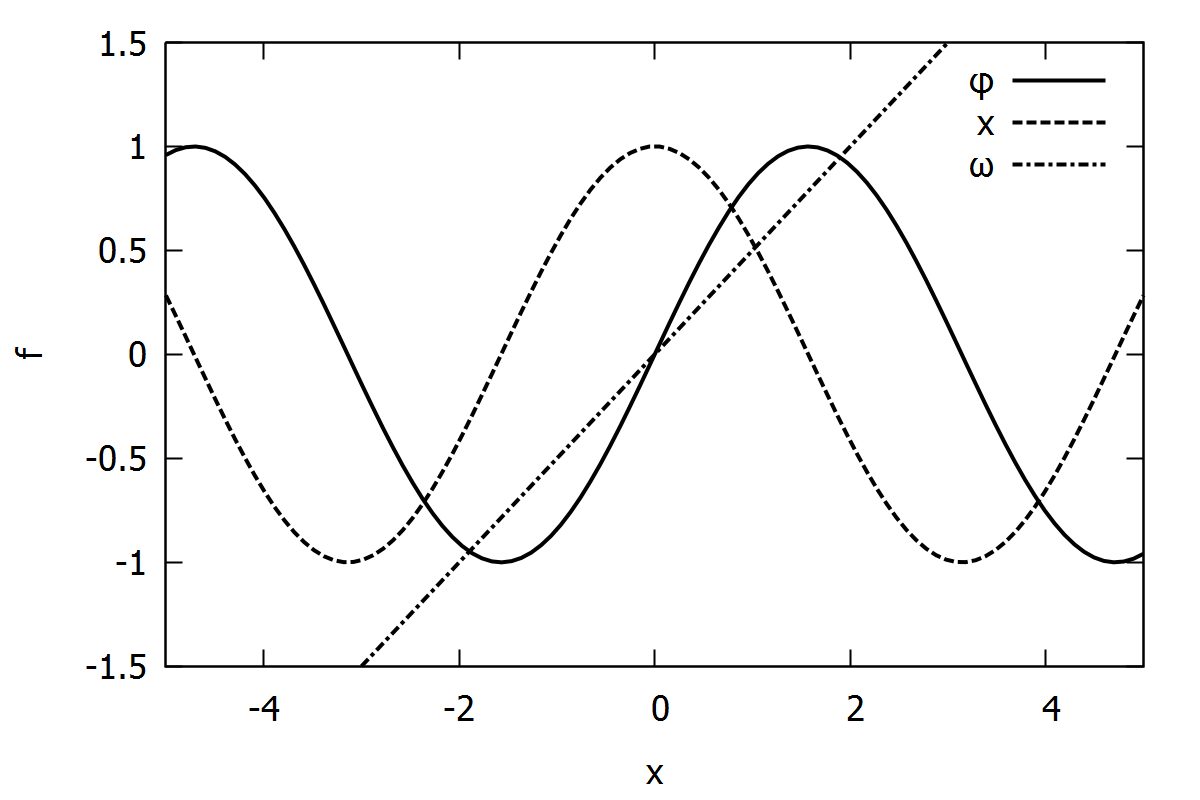
\includegraphics[width=0.95\textwidth]{./gp/custom_lines_style_dashed.png}
\end{frame}

%
%
%
\section{multiplot}
%
%
%

\begin{frame}[t,fragile]
\frametitle{Несколько графиков}
\begin{lstlisting}[basicstyle={\scriptsize}]
set term pngcairo size 1100,800 font "Times,18" linewidth 2
set output 'multiplot1.png'
set multiplot layout 2,2
set xrange [-5:5]
set yrange [-1.5:1.5]
set grid 

set xlabel 'x'
set title 'Синус'
set ylabel 'sin(x)'
plot sin(x) t '' with lines lt -1

set title 'Косинус'
set ylabel 'cos(x)'
plot cos(x) t '' with lines ls 1 

set title 'Тангенс'
set ylabel 'tan(x)'
plot tan(x) t '' with lines ls 2 

set title 'Кубическая парабола'
set ylabel 'x^3'
plot x**3   t '' with lines dt '_' 
\end{lstlisting}
\end{frame}


\begin{frame}[t,fragile]
\frametitle{Несколько графиков}
{\centering
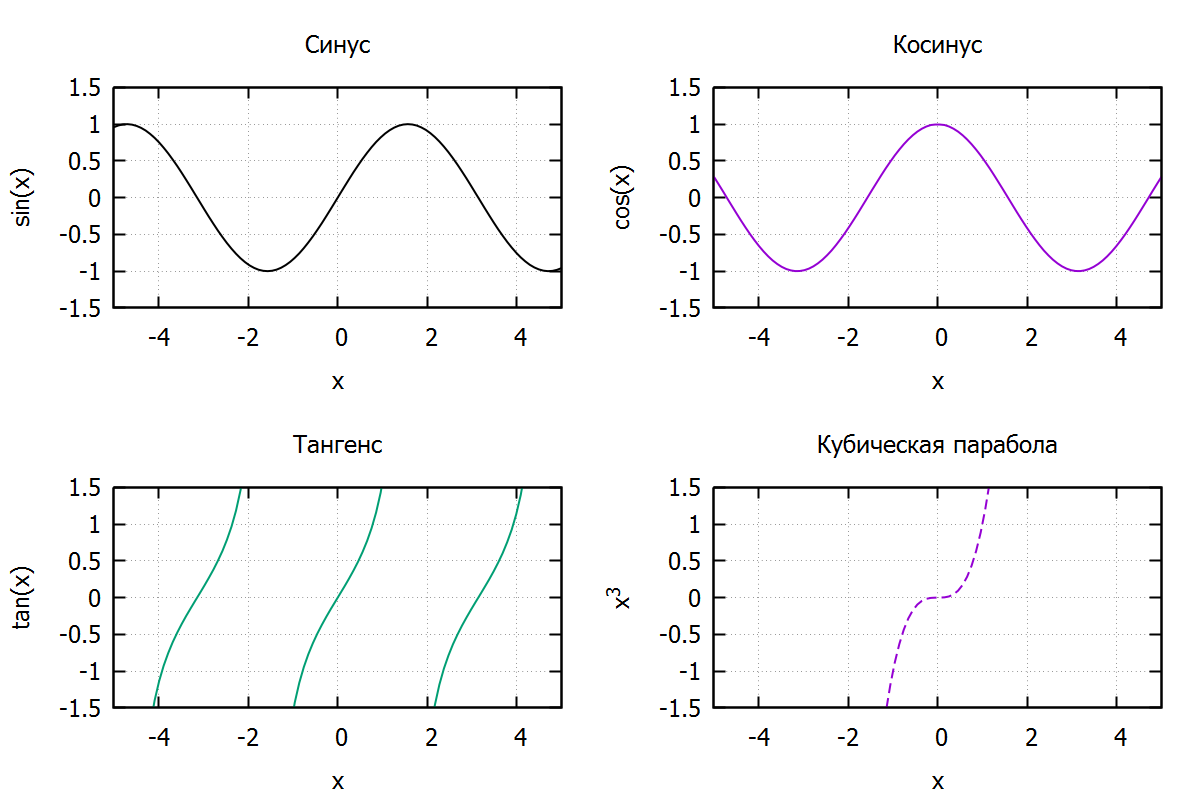
\includegraphics[width=0.95\textwidth]{./gp/multiplot1.png}  
}
\end{frame}




\section{Файлы с данными}

\begin{frame}[c,fragile]
\frametitle{Графики по табличным данным}
Данные в столбац разделены пробелами
\begin{lstlisting}
|\lstcomment{Температура в Самаре (март)}|
|\lstcomment{Минимум, среднее, максимум}|
|\lstcomment{откл. от нормы, осадки мм}|
1   -22.0   -16.0   -10.3 -8.4  0.0
2   -21.7   -15.0   -7.2  -7.6  0.0
3   -19.6   -14.3   -9.5  -7.2  0.0
4   -14.7   -11.1   -6.7  -4.2  6.0
5   -9.2   -3.9  -0.6  +2.8  11.0
6   -14.3   -11.3   -8.0  -4.9  0.3
7   -19.7   -12.9   -7.3  -6.7  0.0
8   -13.0   -10.5   -7.4  -4.6  1.3
...
31  -10.3   -5.9  -1.6  -7.5  0.0
\end{lstlisting}
\end{frame}

\begin{frame}[t,fragile]
\frametitle{График по табличным данным}
\begin{lstlisting}[basicstyle={\scriptsize}]
set term pngcairo size 1200,800 font "Times,26" linewidth 2

set output '04-2018.png'
set xrange [1:31]

set xlabel 'День'
set ylabel |'Температура oС'|
set title  |'Темература в марте 2018 года'|

set key bottom right

plot './temp.txt' using 1:2 t 'мин'  with linespoints ps 2, \
     './temp.txt' using 1:3 t 'сред' with linespoints ps 2, \
     './temp.txt' using 1:4 t 'макс' with linespoints ps 2
\end{lstlisting}  
\end{frame}

\begin{frame}[t]
\frametitle{График}
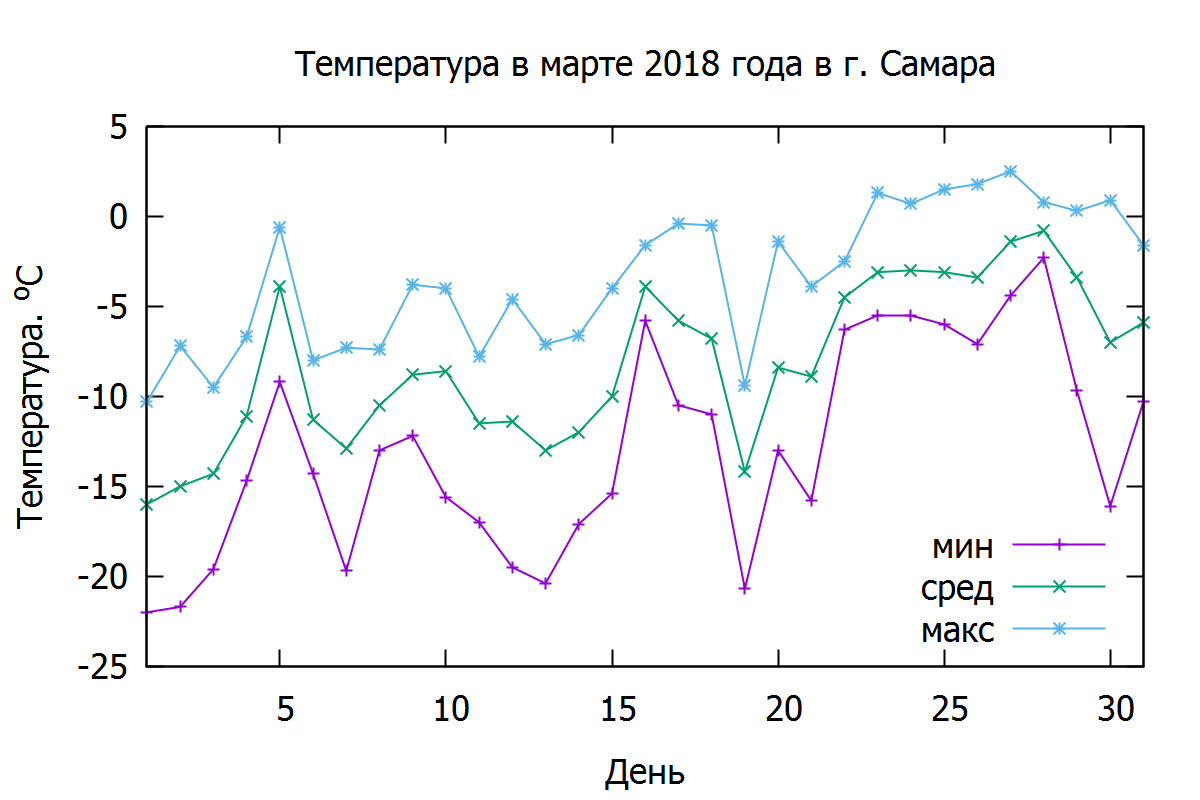
\includegraphics[width=0.95\textwidth]{./gp/04-2018.png}
\end{frame}


\begin{frame}[t,fragile]
\frametitle{Заливка кривых}
\begin{lstlisting}[basicstyle={\scriptsize}]
set term pngcairo size 1200,800 font "Times,26" linewidth 2

set output '04-2018-filled.png'
set xrange [1:31]

set xlabel |'День'|
set ylabel |'Температура oС'|
set title  |'Температура в марте 2018 года в г. Самара'|

set key bottom right

set grid 

set style fill transparent solid 0.25

plot './temp.txt' using 1:3:2 t ''  with filledc lc rgb 'blue', \
     './temp.txt' using 1:3:4 t ''  with filledc lc rgb 'red', \
     './temp.txt' using 1:3   t 'среднее' with lines lc rgb '#2222CC'
\end{lstlisting}  
\end{frame}

\begin{frame}[t]
\frametitle{График}
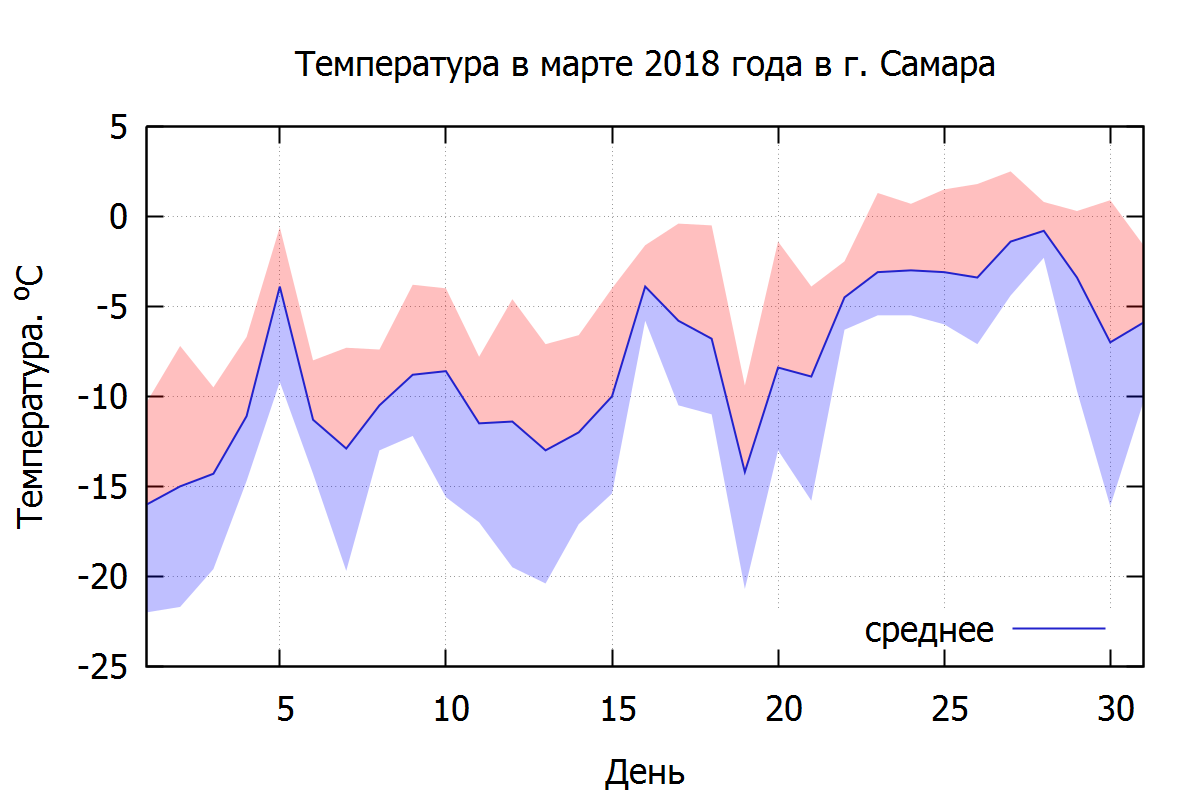
\includegraphics[width=0.95\textwidth]{./gp/04-2018-filled.png}
\end{frame}


\begin{frame}[c,fragile]
\frametitle{Формат файла}
Разделителем столбцов по умолчанию является пробел. Для изменения разделителя используется команда
\begin{lstlisting}[numbers=none]
set datafile separator ','
\end{lstlisting}

\begin{lstlisting}
set term pngcairo size 1200,800 font "Times,22" \
    linewidth 2
|\lstcomment{Разделитель столбцов в файле типа csv}|
set datafile separator ','

set output 'default_data.png'

plot 'motion.csv' u 1:2 t '{/Symbol f}' ,\
     'motion.csv' u 1:3 t 'x' ,\
     'motion.csv' u 1:4 t '{/Symbol w}'
\end{lstlisting}  
\end{frame}


\begin{frame}[t]
\frametitle{График}
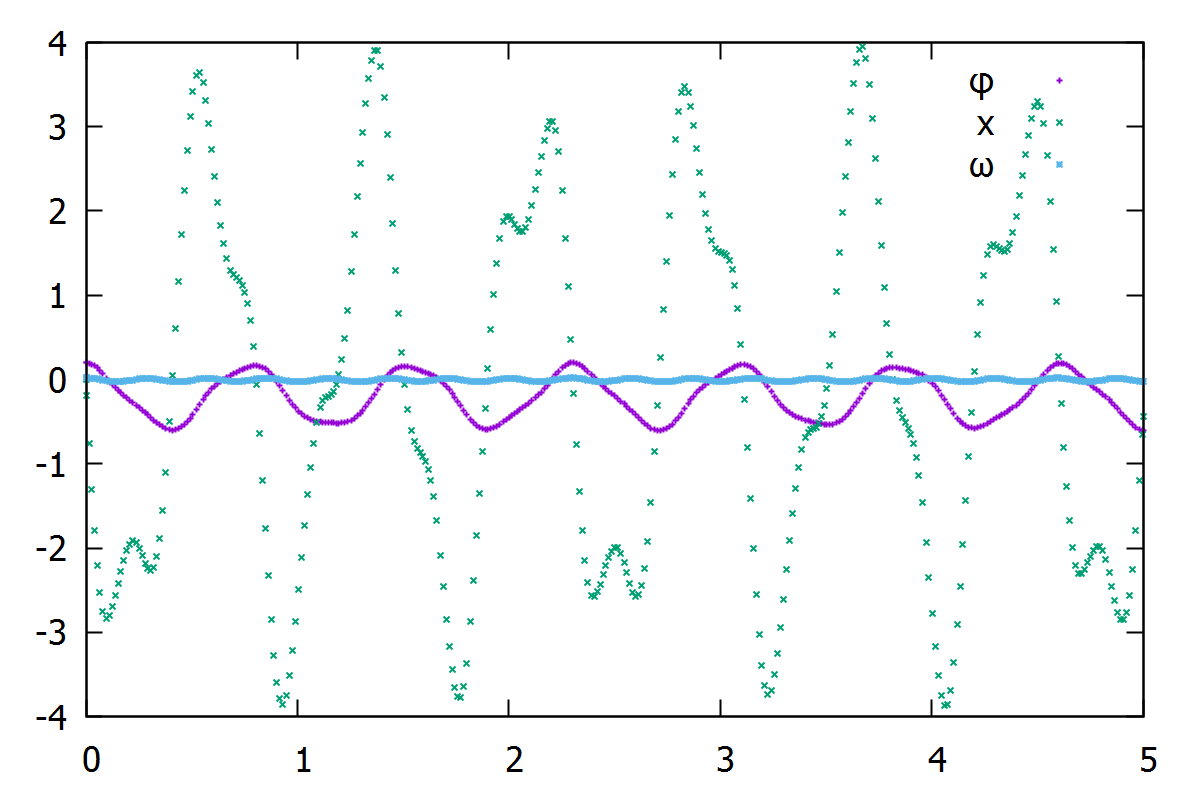
\includegraphics[width=0.95\textwidth]{./gp/default_data.png}
\end{frame}


\begin{frame}[c,fragile]
\frametitle{Тип маркера}
\begin{lstlisting}[basicstyle={\scriptsize}]
set term pngcairo size 1200,800 font "Times,26" linewidth 2

set datafile separator ','
set output 'markers.png'

plot 'motion.csv' u 1:2 t '{/Symbol f}' with linespoints pt 4 ,\
     'motion.csv' u 1:3 t 'x'           with linespoints pt 6 ,\
     'motion.csv' u 1:4 t '{/Symbol w}' with linespoints pt 10
\end{lstlisting}
\end{frame}

\begin{frame}[t,fragile]
\frametitle{Тип маркера}
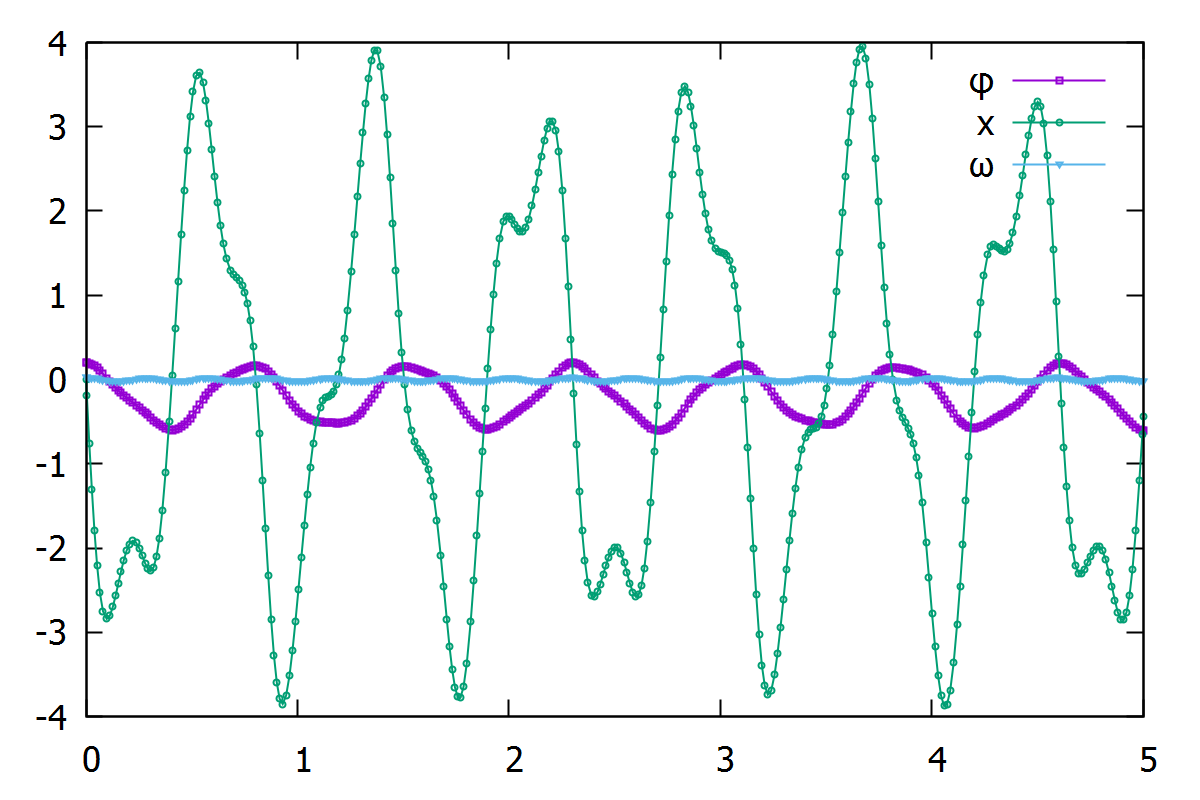
\includegraphics[width=0.95\textwidth]{./gp/markers.png}
\end{frame}


\begin{frame}[c,fragile]
\frametitle{Вычисляемые значения}
\begin{lstlisting}[basicstyle={\scriptsize}]
set term pngcairo size 1200,800 font "Times,26" linewidth 2

set datafile separator ','
set output 'expression.png'
set xlabel |'t, c'|
set ylabel |'Угол поворота, градус'|

plot 'motion.csv' u 1:($2*180/pi) t '' with linespoints pt 4

\end{lstlisting}
\end{frame}

\begin{frame}[t,fragile]
\frametitle{Вычисляемые значения}
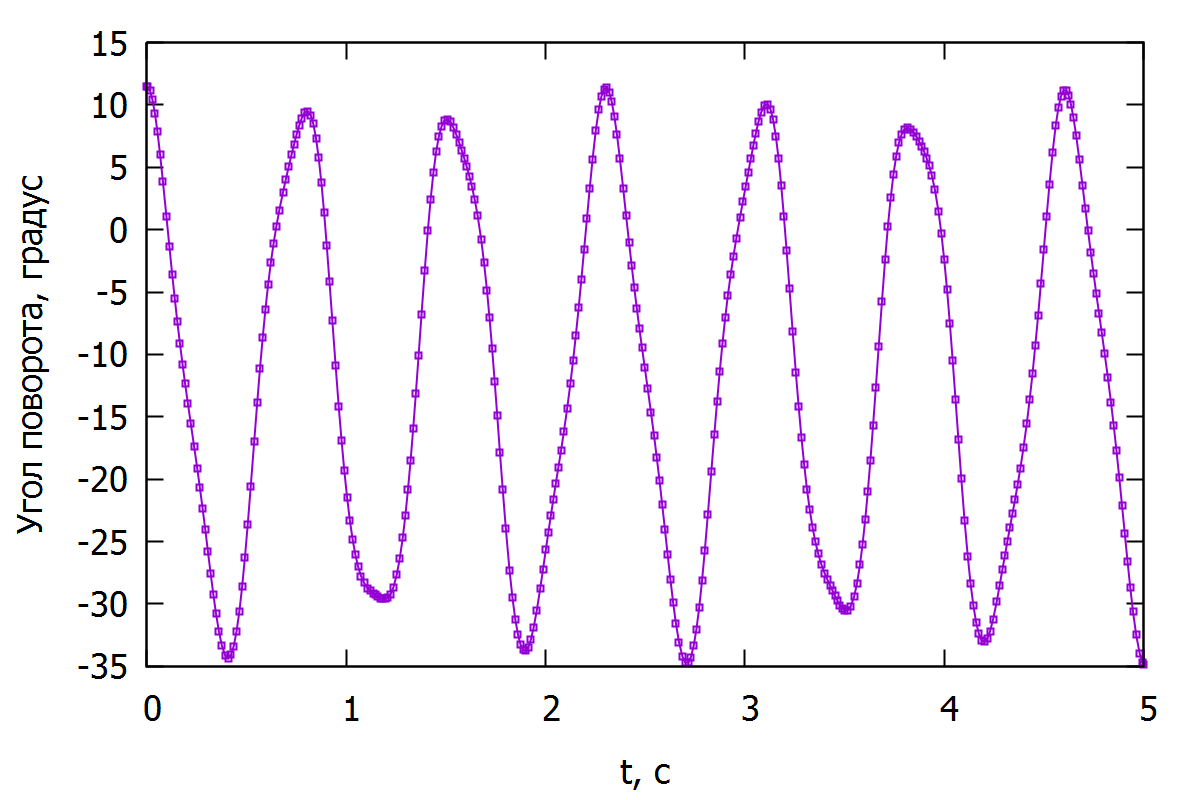
\includegraphics[width=0.95\textwidth]{./gp/expression.png}
\end{frame}


\begin{frame}[c,fragile]
\frametitle{Подписи оси x из файла}
\begin{lstlisting}
|Меркурий|  57910006    0.3871
|Венера|    108199995   0.7232
|Земля|     149599951   1.0000
|Марс|      227939920   1.5236
|Юпитер|    778330257   5.2028
|Сатурн|    1429400028  9.5549
|Уран|      2870989228  19.1913
|Нептун|    4504299579  30.1093
\end{lstlisting}
\end{frame}

\begin{frame}[c,fragile]
\frametitle{Подписи оси x из файла}
\begin{lstlisting}
set term pngcairo size 1200,800 \
    font "Times,24" linewidth 3

set output 'planets.png'
set xrange [*:*]
plot './planets.txt' using 3:xticlabels(1) \
     title '' with linespoints
\end{lstlisting}
\end{frame}

\begin{frame}[t,fragile]
\frametitle{Подписи оси x из файла}
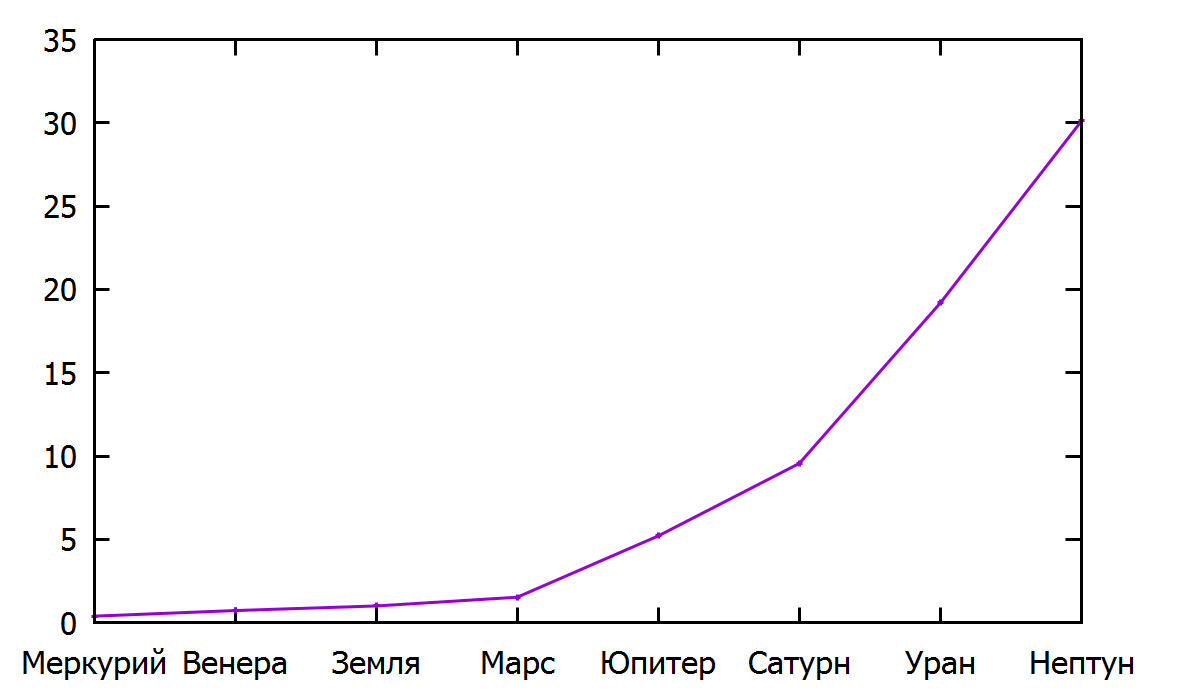
\includegraphics[width=1\textwidth]{./gp/planets.png}
\end{frame}

\begin{frame}[c,fragile]
\frametitle{Логарифмическая шкала y}
\begin{lstlisting}
set term pngcairo size 1200,700 font "Times,24" linewidth 3

set logscale y

set output 'planets_log.png'
set xrange [*:*]
plot './planets.txt' using 3:xticlabels(1) \
     title '' with linespoints ps 2 pt 7
\end{lstlisting}
\end{frame}

\begin{frame}[t,fragile]
\frametitle{Логарифмическая шкала y}
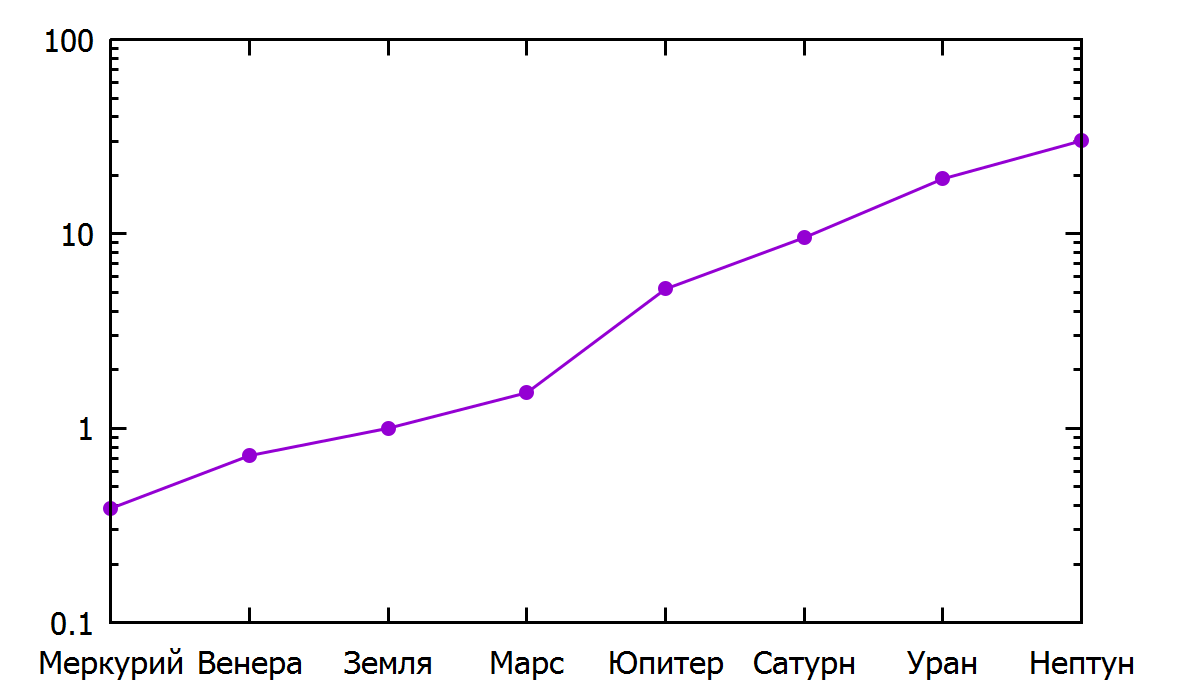
\includegraphics[width=1\textwidth]{./gp/planets_log.png}
\end{frame}


\begin{frame}[c,fragile]
\frametitle{Несколько блоков данных в файле}
Файл blocks.txt. Блоки данных разделяются двумя пустыми строками:
\begin{lstlisting}
|\lstcomment{Первый блок (индекс 0)}|
# X   Y
  1   2
  2   3


|\lstcomment{Второй блок (индекс 1)}|
# X   Y
  3   2
  4   1
\end{lstlisting}  
\end{frame}

\begin{frame}[c,fragile]
\frametitle{Несколько блоков данных в файле}
Данные блока адресуются при помощи директивы \code{index}
\begin{lstlisting}
set term pngcairo size 1200,800 font "Times,18" \
    linewidth 2
set output 'blocks.png'

plot 'blocks.txt' index 0 u 1:2 t 'B1' \
      with linespoints pt 4 ,\
     'blocks.txt' index 1 u 1:2 t 'B2' \
      with linespoints pt 6
\end{lstlisting}  
\end{frame}

\begin{frame}[t,fragile]
\frametitle{Несколько блоков данных в файле}
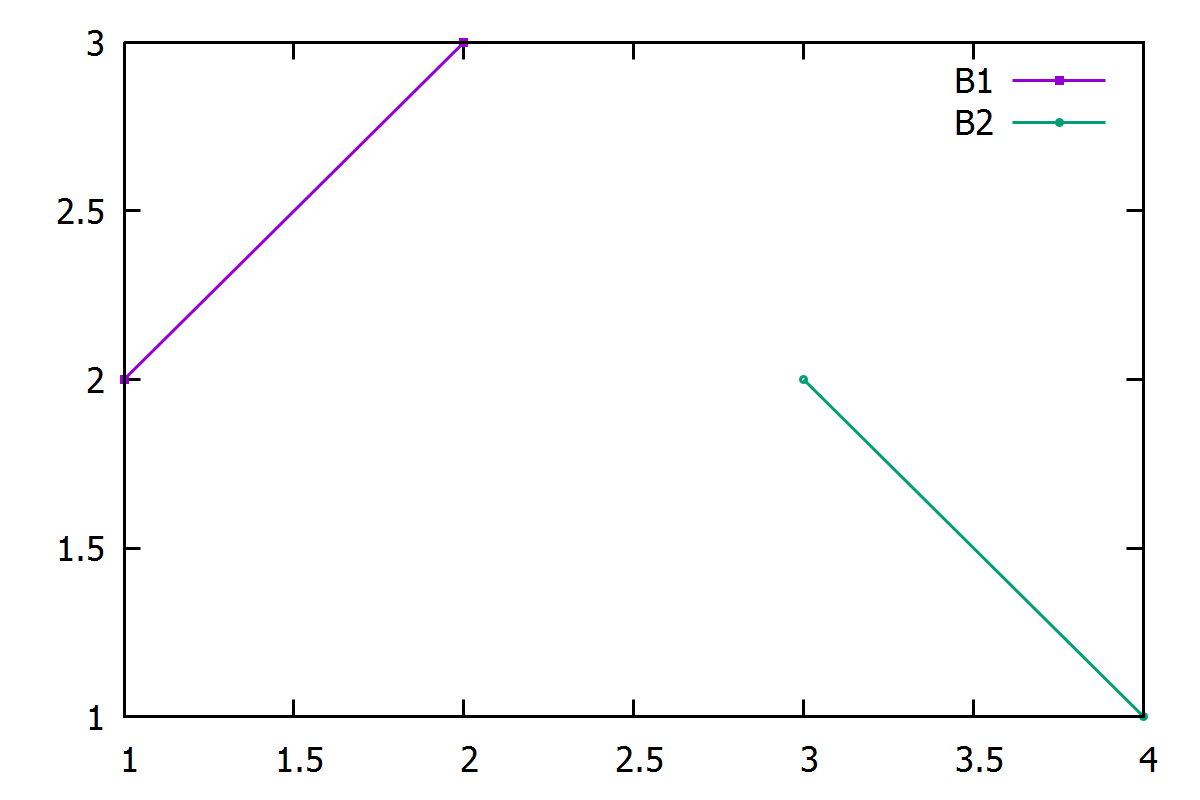
\includegraphics[width=0.95\textwidth]{./gp/blocks.png}
\end{frame}

\begin{frame}[t,fragile]
\frametitle{Две оси y}
\begin{lstlisting}[basicstyle={\scriptsize}]
set term pngcairo size 1200,800 font "Times,24" linewidth 2

set ytics nomirror
set y2tics

set ylabel |'Скорость шарика, м/с'|
set y2label |'Угол (градус), угловая скорость (градус/c)'|

set key top left 
set grid 

set datafile separator ','

set output 'secondary.png'

plot 'motion.csv' u 1:($2*180/pi) t '{/Symbol f}' \ 
                  axes x1y2 with lines lw 2,\
     'motion.csv' u 1:($2*180/pi) t '{/Symbol w}' \
                  axes x1y2 with lines lw 2,\
     'motion.csv' u 1:5 t 'x' axes x1y1 with lines lw 2
\end{lstlisting}
\end{frame}
 
\begin{frame}[t,fragile]
\frametitle{Две оси y}
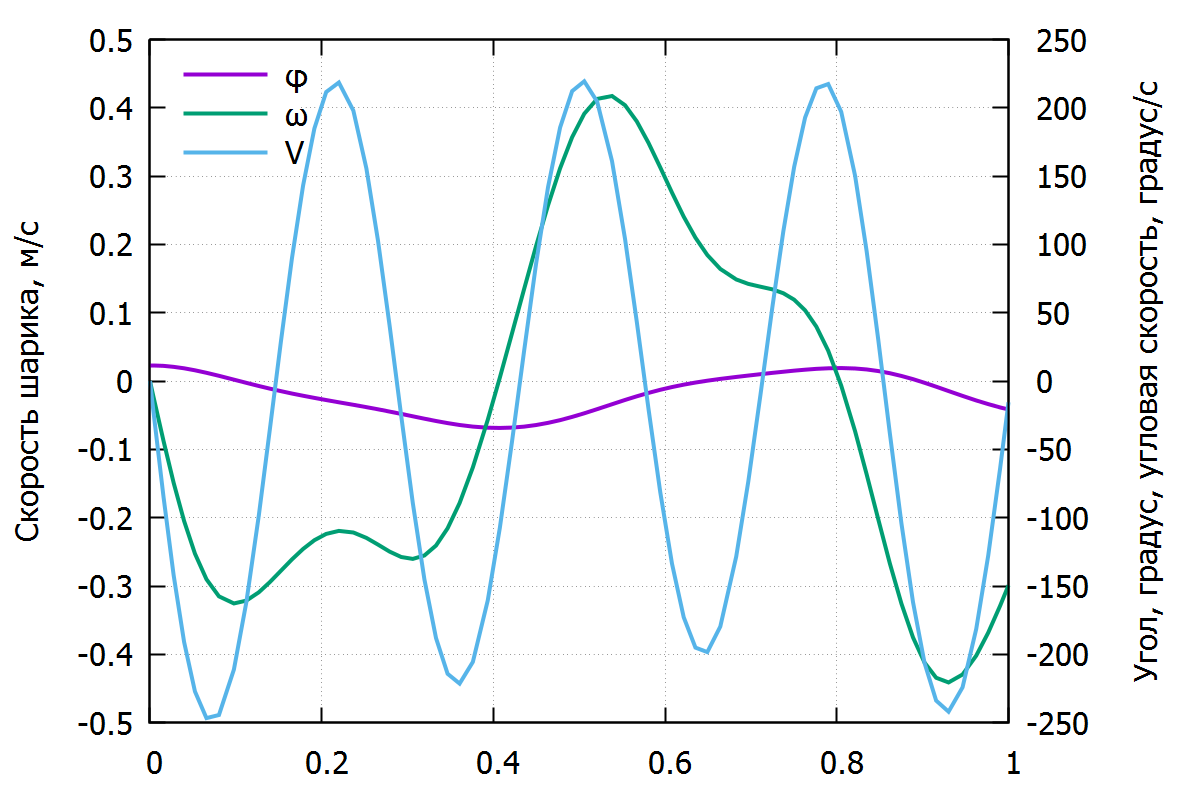
\includegraphics[width=0.95\textwidth]{./gp/secondary.png}
\end{frame}


% \begin{frame}[t,fragile]
% \frametitle{Две оси y}
% \begin{lstlisting}[basicstyle={\scriptsize}]
% set term pngcairo size 1200,800 font "Times,24" linewidth 2

% set ytics nomirror
% set y2tics

% set ylabel  |'Угол поворота, радиан'|
% set y2label |'Угол поворота, градус'|

% set link y2 via y*180.0/pi inverse y*pi/180.0

% set key top left 
% set grid 

% set datafile separator ','

% set output 'secondary_link.png'

% plot 'motion.csv' u 1:($2*180/pi) t '{/Symbol f}' \ 
%                   axes x1y2 with lines lw 2,\
% \end{lstlisting}
% \end{frame}


\section{Задание}

\begin{frame}[t]
\frametitle{Задание}
\begin{itemize}
  \item Установить \emph{gnuplot}
  \item Экспортировать результаты интегрирования движения механимзма (КР) в текстовый файл (время, положение шарика, угол поворота пластины, скорость шарика, угловая скорость пластины).
  \item Построить графики зависимостей от времени всех кинематичеких параметров системы (4 графика на отдельных рисунках в  отдельных файлах).
  \item Построить графики зависимостей от времени всех кинематичеких параметров системы (на одном рисунке).
  \item Построить графики зависимостей от времени всех кинематичеких параметров системы (4 графика на одной странице), используя директиву \emph{multiplot}.
\end{itemize}
  
\end{frame}


 
\end{document}
